The recurrent GSN (RNN-GSN) is an unsupervised, non-probabilistic extension of the deep RNN architecture where the static input distribution is modeled by a GSN and the temporal structure of the input sequence is modeled by an RNN. The basic framework uses RNN hidden states $U$ to output the expected hidden states $\hat{H}$ of a GSN trained over the input distribution $X$, forming an expected input in the sequence $\hat{X}$. This model can be described by the following equations:
\begin{equation}
	\hat{H}_t = \Phi_{h}(A^TU_{t} + b_h)
\end{equation}
\begin{equation}
	\hat{X}_t \sim GSN(X,\hat{H})
\end{equation}
\begin{equation}
	U_{t+1} = \Phi_{u}(B^TX_t + C^TU_t + b_u)
\end{equation}
where \(\Phi_h\) and \(\Phi_u\) are element-wise nonlinear functions,  $A$, $B$, $C$, and $b_u$ are the recurrent network parameters, and $GSN(X,\hat{H})$ is a GSN from Section \ref{gsn} trained with parameters $\Theta_1$ and $\Theta_2$.

This model retains separation between the RNN and the GSN because the RNN hidden states $U$ are only determined by the observed input $x_{t-1}$ and the previous hidden states $U_{t-1}$, as seen in Figure \ref{fig:rnngsn1}. The GSN can be seen as a deep hidden-to-output function for the RNN, reducing the overall complexity that the RNN hidden units $U$ need to model.

\begin{figure}[h!]
  \centering
    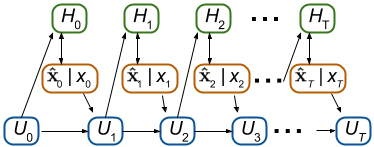
\includegraphics[width=0.5\textwidth]{rnngsn}
\caption{RNN-GSN architecture. Input distribution is X, GSN hidden layers are H, and recurrent hidden units are U.}\label{fig:rnngsn1} 
\end{figure}

\subsection{Initialization strategy}
The initial values of parameters in deep models greatly affect the ability for backpropagation to optimize the overall model \cite{bengio09,initialization}. Because the GSN reduces complexity over the input distribution $X$ independent of the RNN, initializing the GSN parameters first greatly increases the efficiency of training the joint model. This initialization strategy is similar to unsupervised pretraining for layers in the deep RNN, where the GSN is considered a separate layer from the RNN.

For both initialization of the GSN and training the full RNN-GSN model on binary inputs, binary cross-entropy between the expected input $\hat{x}_t$ and observed input $x_t$ is used as the training criteria. Binary cross-entropy is related to the prediction error and is defined as:
\begin{equation}
L(\{x\}) = \frac{1}{T} \sum\limits_{t=1}^T -x_t log(\hat{x}_t) + (1-x_t) log(1-\hat{x}_t)
 \end{equation} 

\subsection{Algorithm}
The RNN-GSN shown in Figure \ref{fig:rnngsn1} and used in the experiments (Section \ref{experiments}) can be trained as follows:
\begin{algorithm}
\caption{RNN-GSN training}\label{algo}
\begin{algorithmic}
	\STATE GSN parameters $\Theta_{GSN} =$ weights $W_{xh}$ and $W_{hh}$, biases $b_x$ and $b_h$, and $k$ walkbacks.
	\STATE RNN parameters $\Theta_{RNN} =$ weights $W_{xu}$, $W_{uu}$, $W_{uh}$, and bias $b_u$.
	\STATE Initialize the GSN:
	\FOR{$x$ in $train\_set$}
		\STATE $predicted\_xs \Leftarrow []$
		\STATE $x_0 \Leftarrow x$
		\STATE $H_0 \Leftarrow 0$
		\FOR{$j=0$ to $k$}
			\STATE $H_{j+1} = W_{xh}x_j + W_{hh}H_{j} + b_h$
			\STATE $\hat{x}_{j+1} = W_{GSN}^T H_{j+1} + b_x$
			\STATE $predicted\_xs$ append $\hat{x}_{j+1}$
			\STATE $x_{j+1}\sim \hat{x}_{j+1}$
		\ENDFOR
		\STATE Perform stochastic gradient descent step for $\Theta_{GSN}$ on binary cross-entropy cost $L(predicted\_xs, x)$.
	\ENDFOR
	\STATE Train the RNN-GSN:
	\STATE $i \Leftarrow 0$
	\STATE $U_0 \Leftarrow 0$
	\FOR{$x$ in $train\_set$}
		\STATE $predicted\_xs \Leftarrow []$
		\STATE $x_0 \Leftarrow x$
		\STATE $H_0 \Leftarrow W_{uh}U_i + b_h$
		\STATE $U_{i+1} = W_{uu}U_i + W_{xu}x + b_u$
		\FOR{$j=0$ to $k$}
			\STATE $H_{j+1} = W_{xh}x_j + W_{hh}H_{j} + b_h$
			\STATE $\hat{x}_{j+1} = W_{GSN}^T H_{j+1} + b_x$
			\STATE $predicted\_xs$ append $\hat{x}_{j+1}$
			\STATE $x_{j+1}\sim \hat{x}_{j+1}$
		\ENDFOR
		\STATE Perform stochastic gradient descent step for $\Theta_{GSN} + \Theta_{RNN}$ on binary cross-entropy cost $L(predicted\_xs, x)$.
		\STATE $i \Leftarrow i+1$
	\ENDFOR
\end{algorithmic}
\end{algorithm}

\subsection{Extending the RNN-GSN to a deeper model}
A natural extension of the RNN-GSN implementation would be to use the GSN to model both the inputs and outputs of the RNN. This new model would form the RNN hidden states $U$ from the GSN hidden states $H$ obtained from the observed input $X$, as well as emit the predicted next hidden states $\hat{H}$ for the GSN. By using a GSN to reduce complexity as both the input-to-hidden and hidden-to-output functions of the RNN, this model greatly increases the efficiency that the RNN units $U$ can learn temporal dependencies of the input. The following equations describe this model:
\begin{equation}
	\hat{H}_t = \Phi_{h}(A^TU_{t} + b_h)
\end{equation}
\begin{equation}
	\hat{X}_t \sim GSN(X,H)
\end{equation}
\begin{equation}
	H_t \sim GSN(X,H)
\end{equation}
\begin{equation}
	U_{t+1} = \Phi_{u}(B^TH_t + C^TU_t + b_u)
\end{equation}
where \(\Phi_h\) and \(\Phi_u\) are element-wise nonlinear functions,  $A$, $B$, $C$, and $b_u$ are the recurrent network parameters, and $GSN(X,\hat{H})$ is a GSN from Section \ref{gsn} trained with parameters $\Theta_1$ and $\Theta_2$.

This structure fully separates the RNN states from the original input $X$, and can be seen in Figure \ref{fig:rnngsn2}.

\begin{figure}[h!]
  \centering
    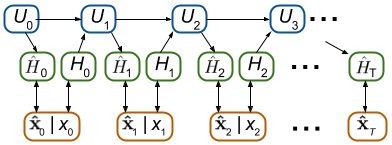
\includegraphics[width=0.5\textwidth]{rnngsn_extension}
\caption{Extension of the RNN-GSN to use both deep input-to-hidden and hidden-to-output functions with a GSN.}\label{fig:rnngsn2}
\end{figure}

Finally, this structure can be theoretically extended to a deeper recurrent model, which we will call a sequence encoding network (SEN). When considering the GSN and RNN as separate layers (Figure \ref{fig:rnngsn2}), they can be alternately stacked to handle arbitrary input and temporal complexity. While combined training would be extremely difficult due to the exploding gradient problem, this model can utilize layer-wise pretraining techniques to first learn input representations and then recurrent relations, continuing as the layers stack. This model combines the input-to-hidden, hidden-to-hidden, hidden-to-output, and stacking aspects of deep RNNs discussed in Section \ref{deep_rnn}.

